% ------ headers globales -------------
\documentclass[12pt, a4paper, twoside]{article}
\usepackage{header}
\usepackage{caratula}
\usepackage{informe}
\addbibresource{informe.bib}
\begin{document}{}
% -------------------------------------



% -- Carátula --
\clearpage{\pagestyle{empty}% parametros para la caratula (caratula.sty)

\materia{Trabajo de Inserción Profesional}
\submateria{Tecnicatura Universitaria en Programación}
\titulo{Mumuki Query Learning}
\subtitulo{Un Runner de SQL para el Proyecto Mumuki}
\fecha{8 de julio de 2017}
\alumno{Leandro Di Lorenzo}{}
\profesor{Ing. Fernando Dodino}{}
%\grupo{}
\maketitle\clearpage}
\setcounter{page}{1}

%-- Índice --
%\clearpage{\pagestyle{empty}\tableofcontents\cleardoublepage}
%\clearpage{\pagestyle{empty}\tableofcontents}

%-- Dentro de TP redefino ciertos comandos para que se pueda compilar todo individualmente --
\begin{TP}


%\setcounter{section}{-1}


%~ Objetivo, introducción.
\section{Introducción}
Hay nuevas formas de aprender a programar, de enseñar a programar
y también nuevas formas de programar. No tiene que ver con gustos or criterios
sino con una realidad. La programación como motor de la computación y
las comunicaciones cambiaron paradigmáticamente la interacción de las
personas y las sociedades a nivel mundial.
Hoy existe una fuerte necesidad de instantaneidad en las respuestas.
En cierto punto se sabe que la respuesta está a la vuelta
\textit{de una googleada}, sólo es necesario indicar las palabras
de búsqueda mágicas.

Esta velocidad de la información repercute en en las prácticas de
la enseñanza formal, la cual necesita moverse por terreno firme
antes que veloz. Cada momento didáctico con un grupo de alumnos
es una oportunidad única de transmisión de conocimiento; y de la
calidad del conocimiento transmitido.
Pero el conocimiento no puede ser transmitido sólo por la calidad del docente.
El alumno tiene que estar dispuesto a aceptar ese conocimiento.

Aprender programación es un desafío en sí mismo. Es necesario poder
manejar herramientas tecnológicas como lenguajes de programación,
entornos de desarrollo, compiladores, intérpretes, etc. Pero también
conceptos como abstracción, refactorización, parametrización.
Los flujos y los protocolos de comunicación, las
estructuras de datos: árboles, listas, pilas, colas, etc.
Y todo sin dejar de tener que cuenta que es necesario ser ordenado y declarativo
en el diseño de programas, pues será leído por otras personas que
tienen que poder entenderlo.

Es fundamental entonces organizar estos conceptos y presentarlos
de forma que no sea abrumadora para el alumno. Es importante poder
minimizar los problemas de una herramienta tecnológicas cuando
se busca enseñar un concepto o una estructura.
Y es importante que el alumno logre sentirse atraído por este conocimiento.

Gran parte de los profresores y alumnos están muy naturalizado con el
uso de ciertas tecnologías (computadoras, celulares, internet, etc.),
las cuales fueron construidas por docentes y profesionales de la programación.
La próxima generación ya usa activamente las herramientas que se busca
enseñarle a construir. Entonces es posible utilizar estas mismas herramientas
para enseñar a construirlas.



\section{Motivación}
La materia \textit{Bases de Datos} contiene mayormente
alumnos en su segundo o tercer semestre en
la Tecnicatura en Programación dictada en la Universidad
Nacional de Quilmes. Idealmente son alumnos que
vienen de cursar las materias \textit{Introducción
a la Programación} y \textit{Organización de Computadoras},
materias antagónicas desde el \textit{alto} y \textit{bajo nivel}
de los conceptos transmitidos. En Intro se aprenden conceptos
de alto nivel usando Gobstones y en Orga conceptos de nivel
de máquina utilizando QSIM\footnote{\url{http://orga.blog.unq.edu.ar/qsim/}}.
Y al mismo tiempo que Bases de Datos muchos cursan
\textit{Programación con Objetos I}.

Desde \textit{BBDD} se busca transmitir el concepto de relación
de información. Se enseñan conceptos como \textit{Modelo de
Entidad-Relacion}, \textit{Normalización} y \textit{Álgebra Relacional}.
El puente entre estos conceptos y el mundo de la programación
es el \textbf{lenguaje SQL}.

Al querer enseñar los conceptos necesarios para que el alumno
pueda manejar SQL, aparecen los problemas recurrentes asociados
a las tecnologías. Los motores utilizados en la industria como
Oracle, Postgres, SQL Server, MySQL, etc., son piezas de software
tan robustas como complejas, y pueden ser una demora cuando se
quieren trasmitir otras ideas fundacionales.

Mumuki cuenta con soporte para Gobstones~\footnote{\url{https://github.com/mumuki/mumuki-gobstones-runner}}~\cite{MumukiGobstonesAloi}
y para QSIM\footnote{\url{https://github.com/mumuki/mumuki-qsim-runner}},
y ambos son utilizados en Intro y Orga respectivamente.
Además de la ventaja de la familiarización de la tecnología,
Mumuki permite incorporar los componentes necesarios para
obtener una adaptación a la necesidad puntual~\footnote{dado que
es Open Source}.


\subsection{Proyecto Mumuki}

\begin{displayquote}[\cite{PaperMumuki}]
``Mumuki es un software educativo para aprender a programar a partir de la resolución de problemas;
plantea enseñar conceptos de programación, en un proceso conducido por guías prácticas
en las que la teoría surge a medida que se avanza. Esta herramienta se presenta al
estudiante como una aplicación Web interactiva, en la que se articulan explicaciones
y ejemplos con la opción de que cada uno realice su propia solución y la plataforma
la pruebe y corrija instantáneamente, orientando acerca de los aciertos y errores.''
\end{displayquote}

Mumuki es el resultado del trabajo de muchas personas que creen
que es necesario plantear nuevas formas de enseñar a programar.
Lo que se plantea es un complemento a la clase en el aula, no
un reemplazo, pero haciendo foco en que la plataforma pueda ayudar
a resolver el mayor número de \textit{problemas técnicos}
que el alumno pueda tener con la tecnología y permitir al docente enfocarse
en las problemáticas inherentes a la enseñanza de los conceptos.

Es común en cursos introductorios de programación orientada a objetos que los alumnos
estén una o dos clases (y el tiempo entre semana) tratando de hacer funcionar
el entorno de Java con sus bibliotecas y el IDE, en lugar de
aprovechar ese tiempo para practicar conceptos elementales como mensajes
entre objetos, comportamiento, herencia, etc.

Al usar una plataforma como Mumuki el docente puede saltear esta problemática
y enforcarse en lo conceptual. Por supuesto que todo estudiante de programación
debe lograr aprender a instalar y configurar entornos de desarrollo, pero
en ciertos niveles esta nueva forma de enseñar evita muchas
frustaciones puramente inherentes a la tecnología,
las que sino terminan por ser asociadas a la programación como un todo.

\subsection{Gobstones como hilo conductor}

Si bien este trabajo no se relaciona directamente con Gobstones
\footnote{\url{http://www.gobstones.org/}},
gran parte de las ideas utilizadas tienen como uno
de los orígenes las planteadas en el libro
\enquote{Las bases conceptuales de la Programación: Una nueva forma de aprender a programar}~\cite{LibroGobstones}, del cual obtenemos su definición:

\begin{displayquote}
``Gobstones es un lenguaje conciso de sintaxis razonablemente simple,
orientado a personas que no tienen conocimientos previos en programación.
El lenguaje maneja distintos componentes propios, ideados con el fin de
aprender a resolver problemas en programación,  pero al mismo tiempo
intentando volver atractivo el aprendizaje, para lograr captar la atención
y capacidad de asombro del estudiante.''
\end{displayquote}

Gobstones busca facilitar la enseñanza de conceptos iniciales de programación
tratando de mantener distancia de las problemáticas técnicas y
la comprensión de errores complejos ante fallos de programas.
Cuenta con el entorno \textit{PyGobstones}~\footnote{\url{http://inpr.web.unq.edu.ar/instalacion-de-pygobstones/}} programado en python
pero actualmente se está desarrollando una versión web~\footnote{\url{https://gobstones.github.io/editor-beta/}} que no requiere instalación.




\section{Presentación}\documentclass{beamer}
\usepackage{packages}
\graphicspath{ {./imgs/}{../imgs/} }

% \usetheme{AnnArbor}
\usetheme{Warsaw}
\usecolortheme{beaver}
\useoutertheme{miniframes}
\setbeamertemplate{headline}{}
\setbeamertemplate{title page}[default][rounded=true]
\setbeamertemplate{frametitle}[default][colsep=0bp,rounded=false,shadow=false]
\setbeamercolor{frametitle}{bg=beaverdarkred,fg=white}
\setbeamercolor{framesubtitle}{bg=darkunq}
\setbeamercolor{title}{fg=beaverdarkred}
\setbeamercolor{subtitle}{fg=beaverdarkred}
\setbeamercolor{author in head/foot}{fg=beaverdarkred,bg=darkgrey}
\setbeamertemplate{footline}
{
    \leavevmode%
    \hbox{%
    \begin{beamercolorbox}[wd=1\paperwidth,ht=2.25ex,dp=1ex,center]{title in head/foot}%
        \usebeamerfont{title in head/foot}\insertshortauthor\insertshorttitle\hspace*{2em}
    \end{beamercolorbox}}%
    \vskip0pt%
}
\setbeamertemplate{itemize item}[triangle]
\setitemize{label=\usebeamerfont*{itemize item}%
  \usebeamercolor[fg]{itemize item}
  \usebeamertemplate{itemize item}}




\title[\texttt{ UNQ -> TIP -> MQL}]{Mumuki Query Learning}
\subtitle{\emph{Un Runner de SQL para el Proyecto Mumuki}}

\titlegraphic{
    
\includegraphics[width=.4\textwidth]{logo-unq}
}

\author[\texttt{Leandro Di Lorenzo ::}]
{
    Leandro~Di~Lorenzo \\
    \textbf{Coordinador:} Ing. Fernando Dodino
    % \vspace{-1em}
}


\institute[TIP - UNQ]
{
   \textsc{
       \small{Tecnicatura en Programación Informática}
   }
}

\date[jul 2017]{8 de Julio, 2017}


\makeatletter
    \newenvironment{withoutheadline}{
        \setbeamertemplate{headline}[default]
        \def\beamer@entrycode{\vspace*{-\headheight}}
    }{}
\makeatother



\begin{document}



%%
%% Carátula
%%
\begin{frame}[plain]
    \vspace{2em}
    \titlepage
    \vspace{-2em}
    \begin{figure}[h]
        
\includegraphics[width=.3\textwidth]{logo-unq}
    \end{figure}
\end{frame}


%%
%% Idea: MQL
%%
\begin{frame}{Idea: MQL}
    \begin{figure}[h]
        
\includegraphics[scale=1]{logo-mql}
    \end{figure}
\end{frame}


%%
%% Proyecto Mumuki
%%
\begin{frame}{Proyecto Mumuki}
    \begin{figure}[h]
        
\includegraphics[width=1\textwidth]{proyecto-mumuki}
    \end{figure}
\end{frame}


%%
%% Un poco de data...
%%
\begin{frame}{Un poco de data...}
    \begin{itemize}%[<+->]
        \item Mumuki es una plataforma educativa para la enseñanza de programación, y es \textit{Open Source}.
        \item Se puede utilizar de forma autodidacta o como aula virtual con seguimiento.
        \item Es desarrollada y mantenida por estudiantes y docentes de varias universidades públicas, incluída la UNQ.
        \item Está siendo utilizada en diferentes entidades educativas del país.
        \item Tiene un enfoque didáctico con fuerte incapié en los conceptos por sobre las tecnologías.
    \end{itemize}
\end{frame}


%%
%% Mumuki :: Ejercicios
%%
\begin{frame}{Mumuki :: Ejercicios}
    \begin{figure}[h]
        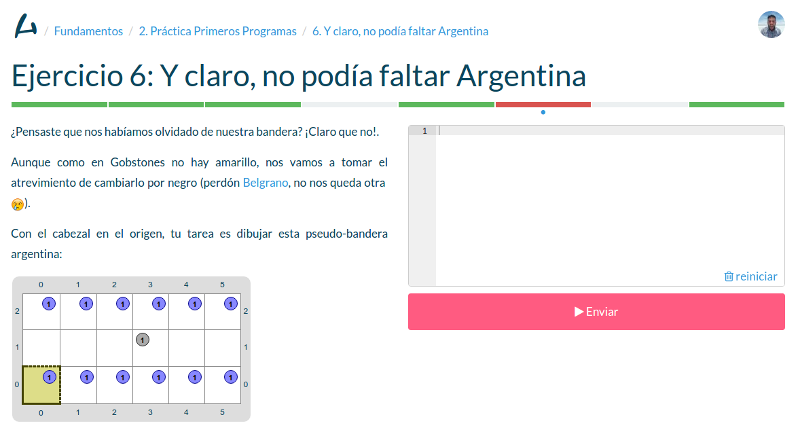
\includegraphics[width=1\textwidth]{gobstones-exercise}
    \end{figure}
\end{frame}

%%
%% Mumuki :: Corrección Automatizada
%%
\begin{frame}{Mumuki :: Corrección Automatizada}
    \begin{figure}[h]
        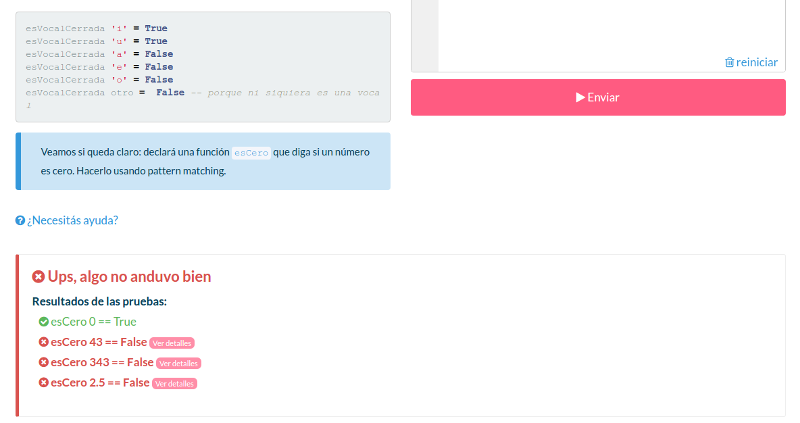
\includegraphics[width=1\textwidth]{haskell-ups}
    \end{figure}
\end{frame}

%%
%% Mumuki :: Seguimiento
%%
\begin{frame}{Mumuki :: Seguimiento}
    \begin{figure}[h]
        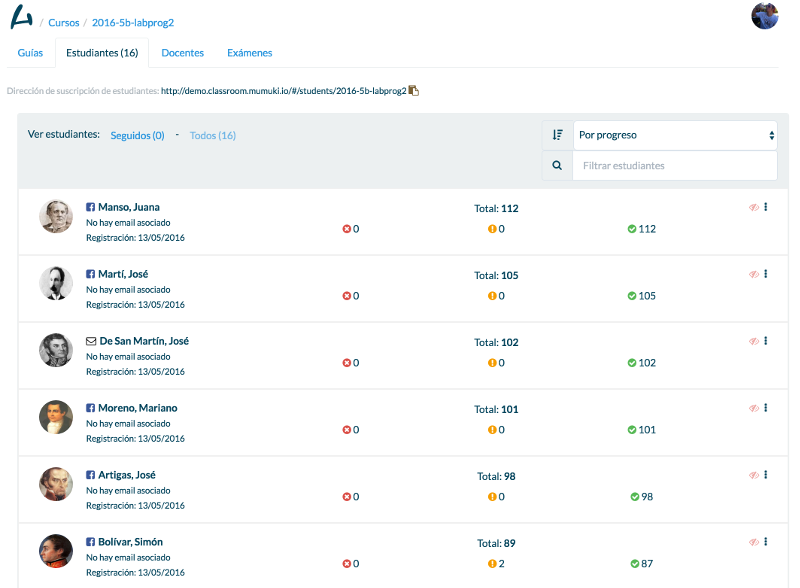
\includegraphics[width=1\textwidth]{classroom-students}
    \end{figure}
\end{frame}


%%
%% Mumuki :: Versionado
%%
\begin{frame}{Mumuki :: Versionado}
    \begin{figure}[h]
        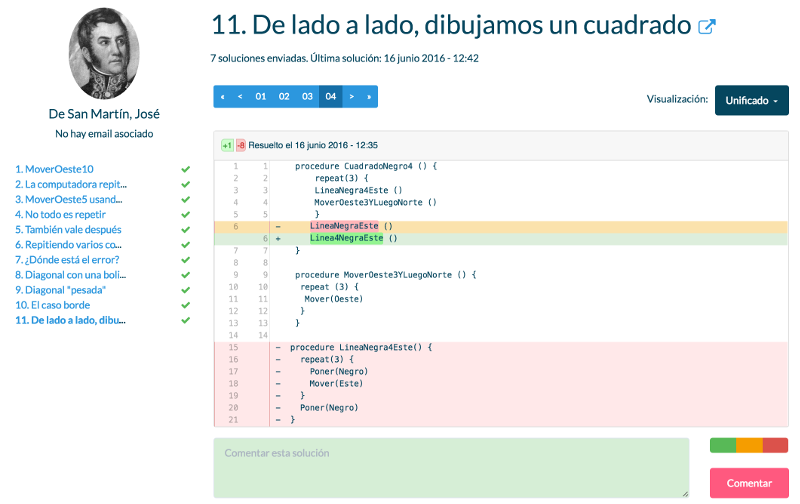
\includegraphics[width=1\textwidth]{classroom-student-detail}
    \end{figure}
\end{frame}


%%
%% Mumuki :: Contenido Personalizable
%%
\begin{frame}{Mumuki :: Contenido Personalizable}
    \begin{figure}[h]
        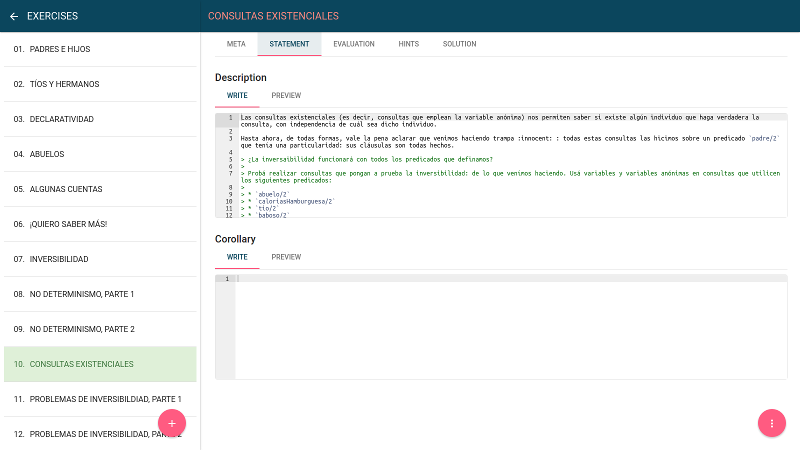
\includegraphics[width=1\textwidth]{editor}
    \end{figure}
\end{frame}


%%
%% Mumuki :: Contenido Actual
%%
\begin{frame}{Mumuki :: Contenido Actual}
    \begin{figure}[h]
        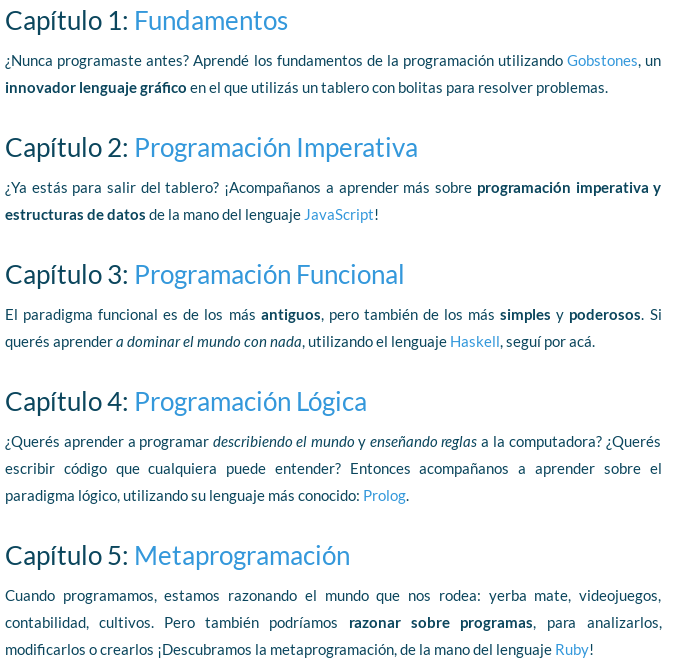
\includegraphics[width=.85\textheight]{contenido}
    \end{figure}
\end{frame}


%%
%% Mumuki Query Learning :: Objetivos
%%
\begin{frame}{Mumuki Query Learning :: Objetivos}

    Proveer a los docentes de \textit{Bases de Datos} una herramienta para:

    \begin{itemize}
        \item Mejorar la didáctica en la enseñanza de conceptos de SQL
        \item Facilitar el seguimiento del aprendizaje de los alumnos
        \item Contar con mejores elementos de evaluación
    \end{itemize}

    \vspace{1em}

    Proveer a los alumnos una herramienta para:

    \begin{itemize}
        \item Comprender mejor los conceptos recibidos
        \item Recibir feedback de forma temprana
        \item Poder analizar por su cuenta los fallos obtenidos para poder aprender de ellos
        \item Analizar su propio progreso visualizando los pasos dados hasta la resolución de los problemas
    \end{itemize}
\end{frame}

%%
%% Consecuencias Deseadas
%%
\begin{frame}{MQL :: Consecuencias Deseadas}

    \begin{itemize}
        \setlength\itemsep{1em}
        \item Aportar al crecimiento del \textit{Proyecto Mumuki} con una nueva tecnología de aprendizaje.
        \item Ayudar a todo programador que desee mejorar su capacidad y calidad en
        relación al uso de las bases de datos relaciones.
        \item Dejar abierta la posibilidad de extensión hacia:
        \vspace{.4em}
        \begin{itemize}
            \setlength\itemsep{.5em}
            \item Álgebra Relacional
            \item Bases de datos no relaciones (MongoDB, Neo4j, Redis, etc...)
        \end{itemize}
    \end{itemize}

\end{frame}


%%
%% Herramientas a Implementar
%%
\begin{frame}{MQL :: Herramientas a Implementar}
    \begin{itemize}%[<+->]
        \setlength\itemsep{1em}
        \item Docker container con PostgreSQL o SQLite
        \item Runner de SQL en Ruby que permita:
        \vspace{.4em}
        \begin{itemize}
            \setlength\itemsep{.5em}
            \item Obtener y ejecutar el código SQL recibido
            \item Validar resultados obtenidos contra esperados
            \item Analizar sintaxis para exponer buenas prácticas de código
        \end{itemize}
        \item Classroom con set de ejercicios
    \end{itemize}
\end{frame}


%%
%% Mumuki :: Organizaciones que la utilizan
%%
\begin{frame}{Mumuki :: Organizaciones que la utilizan}
    \begin{figure}[h]
        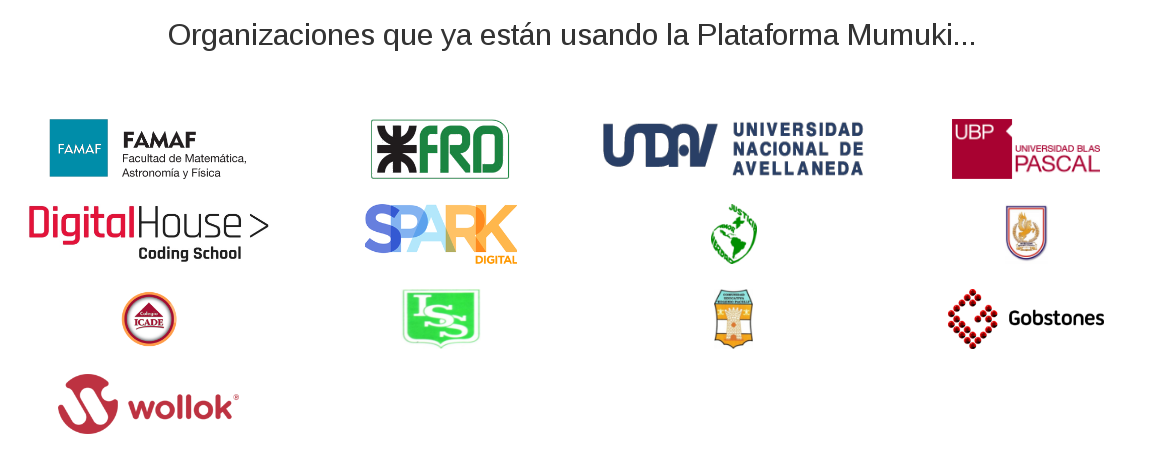
\includegraphics[width=1\textwidth]{organizaciones}
    \end{figure}
\end{frame}


%%
%% Algunos Links
%%
\begin{frame}{Algunos Links}
    \begin{itemize}%[<+->]
        \setlength\itemsep{.7em}
        \item Proyecto Mumuki: \url{http://www.mumuki.org/}
        \item Plataforma: \url{https://mumuki.io/}
        \item Código en GitHub: \url{https://github.com/mumuki}
        \item Nota en Télam: \url{http://www.telam.com.ar/notas/201703/183460-mumuki-plataforma-gratuita-programacion\\-aprendizaje-ensenanza-software.html}
        \item PostgreSQL: \url{https://www.postgresql.org/}
        \item SQLite: \url{https://www.sqlite.org/}
        \item Docker: \url{https://www.docker.com/}
    \end{itemize}
\end{frame}


%%
%% Gracias :: Preguntas
%%
\begin{frame}[plain]
    \begin{center}
        \begin{figure}[h]
            
\includegraphics[scale=.7]{questions}
        \end{figure}
        \vspace{2em}
        \Large{¿Preguntas, ideas, comentarios?}
    \end{center}
\end{frame}

\end{document}


\section{Alcance y Trabajo futuro}
Inicialmente este trabajo busca lograr establecer guías de
estudio de SQL como parte de los contenido de la materia \textit{Bases de Datos}.
Pero al ser parte de un proyecto \textit{Open Source}, se espera
que pueda servir como mejora en todo ámbito que sea posible
la enseñanza de SQL y de Bases de Datos Relaciones.

Al mismo tiempo queda planteado el desafío de lograr
herramientas que cubran una superficie mayor de los conceptos
de Bases de Datos. Un \textit{Runner de Álgebra Relacional}
sería un complemento ideal. Al ser \textit{SQLite} poco
estricto con algunas restricciones de datos, podrían
ser útil contrar con un \textit{Runner} que permita
establecer \textbf{transacciones} y eventualmente interrumpirlas
para analizar comportamiento.
Las Bases de Datos No Relaciones son un buen desafío
también para enseñar \textit{mongoDB}, \textit{Neo4j}, etc.


\section{Conclusiones}


%\clearpage
\printbibliography


\end{TP}
\end{document}
